\documentclass[12pt]{article}
\usepackage{graphicx}
\author{Manuel González González}
\title{Práctica 7: Perceptrón multicapa}
\begin{document}
\maketitle

\section*{Ejercicio 2}
\subsection*{a)}
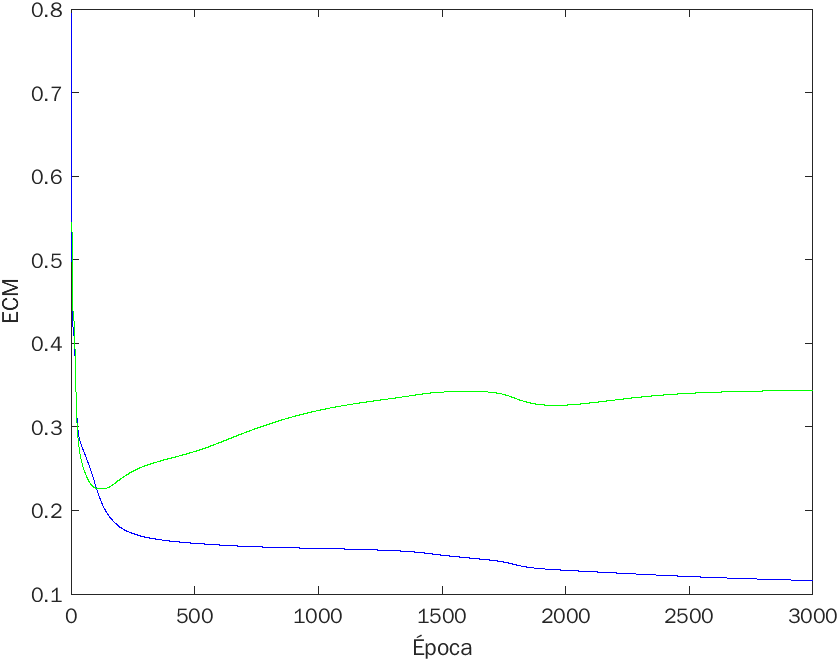
\includegraphics[scale=1]{2a.png}

\subsection*{b)}
Debería de parar en la época en la que se encuentra el primer mínimo local de validación. Esto se debe a que es el primer punto en el que el error entre el conjunto de entrenamiento y validación es menor.

\subsection*{c)}
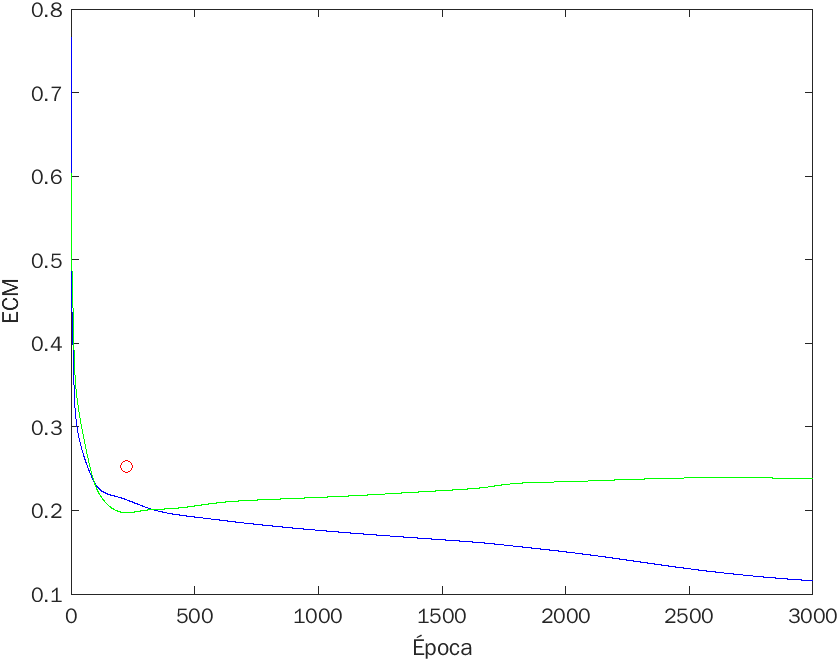
\includegraphics[scale=1]{2c.png}

\subsection*{d)}
El comportamiento varía en cada ejecución. Esto ocurre ya que los conjuntos de entrenamiento y validación se eligen de forma aleatoria y en el proceso de ejecución no se reproduce la misma secuencia de valores. Por ello los mínimos locales que se encuentran son distintos.

\begin{figure}
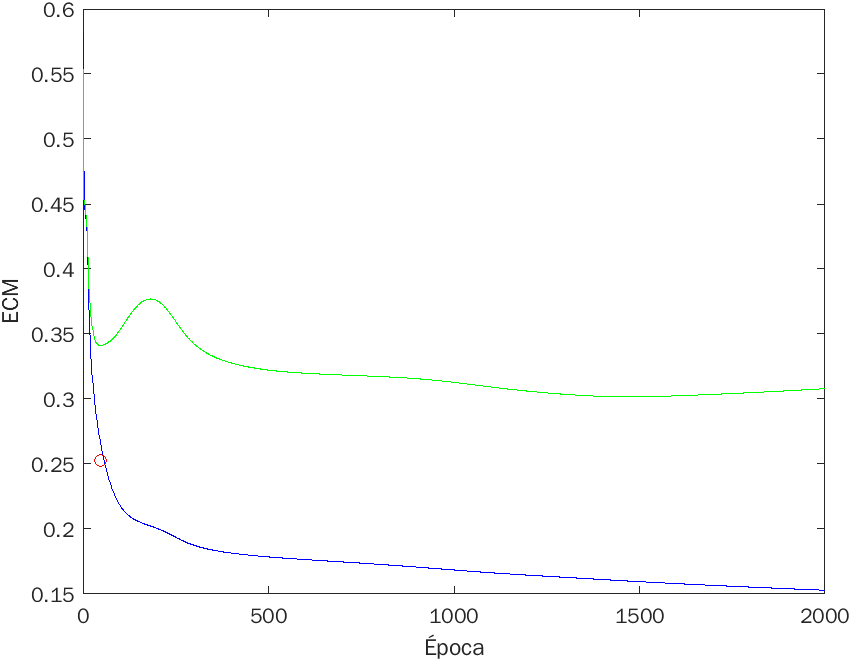
\includegraphics[scale=1]{2d1.png}
\caption{Primera ejecución}
\end{figure}
\begin{figure}
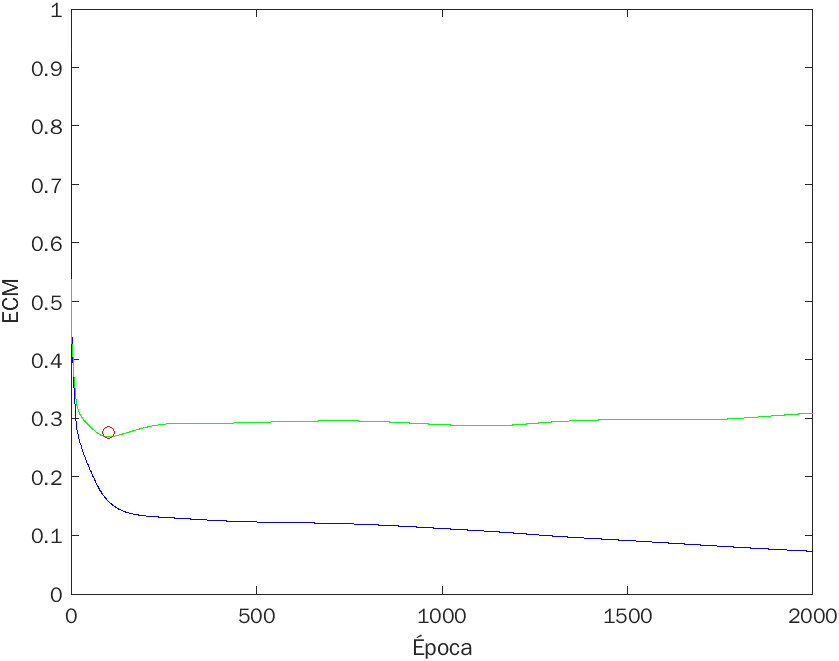
\includegraphics[scale=1]{2d2.png}
\caption{Segunda ejecución}
\end{figure}
\begin{figure}
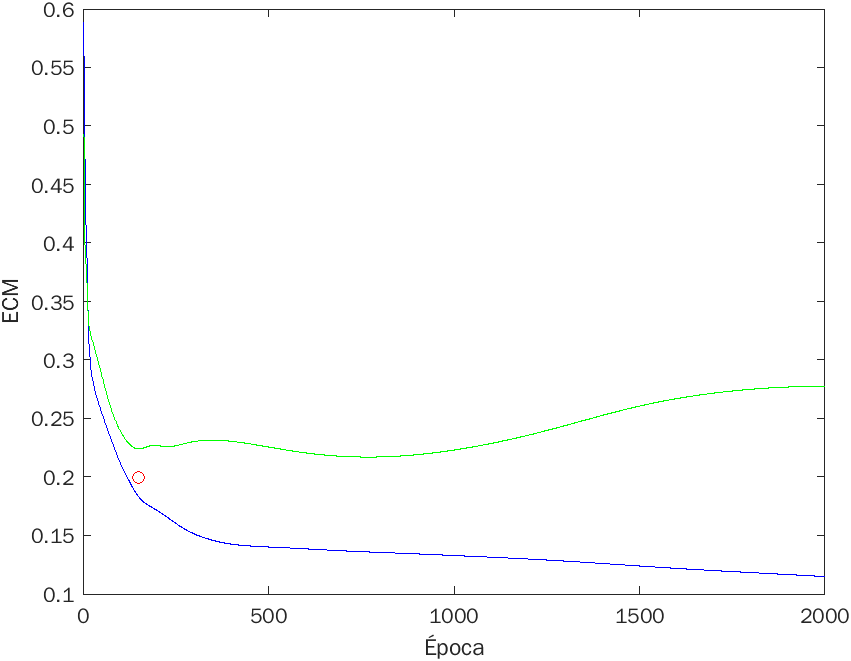
\includegraphics[scale=1]{2d3.png}
\caption{Tercera ejecución}
\end{figure}


\subsection*{e)}
El rango de la función a aprender son los valores 0 y 1.

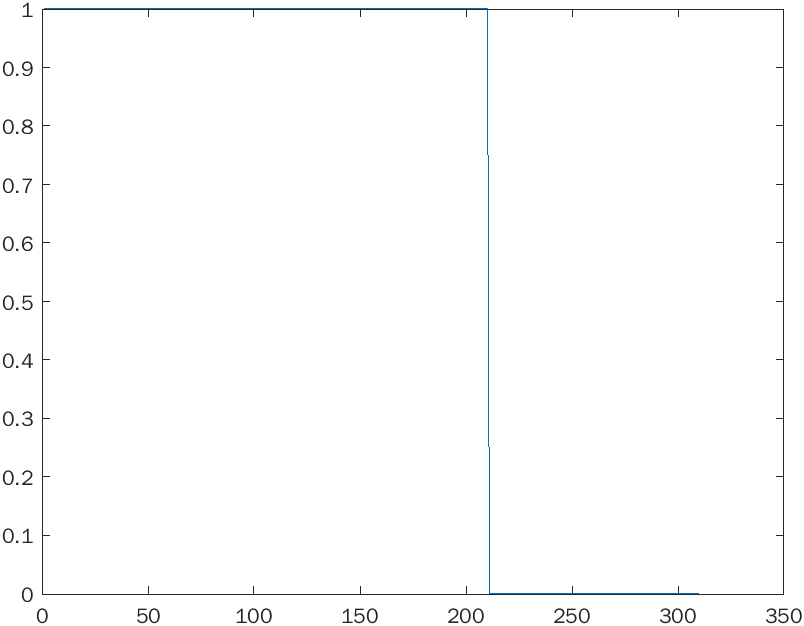
\includegraphics[scale=1]{2e.png}

\end{document}